\section{Communication}
\label{sec:communication}

Communication is an important topic in YARP, since
we assume the robot is controlled by a pool of networked PCs.  This is currently
necessary for any robot doing signicant perceptual processing; for
example object recognition {\em and} face detection {\em and}
responsive motor control.  We do not assume those machines run the
same operating system, since the availability of device drivers and
can force such choices.

Communication in YARP follows the {\em Observer} pattern~\cite{gamma95design}.  The state
of special {\it Port} objects can be delivered to any number of
observers, in any number of processes distributed across any number of
machines.  YARP manages these connections in a way that insulates
the observed from the observer and, just as importantly, insulates
observers from each other.  For example,
if one observer reads a data source slowly and infrequently, this
does not force other observers to slow down.

The basic YARP module is an IPC infrastructure that supports communication across a
network exploiting different protocols. YARP allows interconnecting many modules
seamlessly without subscribing to any specific programming style, language interface, 
or demanding specifications as for instance in CORBA~\cite{vinoski97corba} or DCOM [ref]. That is, YARP 
is a plain library linked to user-level code and as such migration to YARP can be easily
carried out a posteriori. 

Systems such as the already mentioned CORBA, although far more powerful than YARP, require 
adhering to well-defined interface specificiations (nothing bad as such) but consequently 
their link between the general algorithmic code and the communication layer is much 
stricter. 

We have taken a more lightweight approach: any C++ code can use YARP directly just by 
instantiating communication classes. Other programming languages can access YARP as well, 
provided they have means of linking and calling C++ code. We have successfully used YARP 
from within Matlab or L~\cite{brooks90behavior}.

Communication channels in YARP can be connected either programmatically or at run-time.
Each communication object, described next, can receive commands from other processes and 
react consequently by activating or removing a specific connection.

The communication abstraction is called a ``port''. The port is an active object managing
multiple connections for a given data type either as input or output (see figure \ref{fig:port}). Each connection has
a state that can be manipulated by certain commands, which manage the connection or obtain
state information from it. Although a port can behave both as input and output, the 
user interface, for convenience, enforces only one direction. An input port can receive 
from multiple connections at different data rates ``speaking'' different protocols
(e.g. TCP, UDP, multicast). An output port can send data to many destinations reading at
different rates on different protocols. Service channels are also temporarily created to
perform the handshaking between ports; in this case the protocol of choice is TCP for
reliability. The use of several different protocol allows to exploit at best their 
characteristics:
\begin{itemize} \pflist
	\item TCP: reliable, it can be used to guarantee the reception of a message;
	\item UDP: faster than TCP, used for point to point connections;
	\item multicast: used for creating one to many connections, efficient for distributing
	the same information to many targets;
	\item shared memory: employed for local connections (transparently invoked by the port
	code);
	\item QNet: a fast and synchronous protocol used under the QNX real-time OS.
\end{itemize}

Communication is fully asynchronous and as such messages are not guaranteed to be 
delivered unless special provisions are made. The most natural semantic for YARP ports is
thus that of dealing with recurrent messages, updated and sent often enough, where losing 
one message does not compromise the integrity of the system. This is tailored at
sensorial data that are generated periodically: e.g. images and sound. YARP is definitely
not an event based system since a single message is not guaranteed to get through. A
typical application is, for example, the acquisition of images, and delivery to many 
machines performing the processing in parallel. Slower processes might simply not
use all the available frames in the stream of data and rather skip some of them.

\begin{figure}
	\centering
		\includegraphics[width=8.5cm]{port.eps}
	\caption{The port internal structure: in practice either input or output connections
	are used for a given instance of a port object.}
	\label{fig:port}
\end{figure}

More recently, at the cost of bidirectional synchronization, a method for guaranteeing
the delivery of messages has been added but this is not the most straightforward and
natural use of ports.

Reading from ports can be blocking, non-blocking (polling), or can happen on a callback.
Writing is normally non-blocking, although it can be made to block depending on the requirements of the channel. In short, once data is available, a reference to a data
buffer (of the same type of the data being received) is returned to the user code. This
remains valid for the user to manipulate it as long as no other calls to the read function
are made. 
On a write, on the other hand, the buffer is passed to the trasmission code which deals
with the details of the communication, while user code can continue execution.

Ports are located on the network by symbolic names which are managed by a name server
(the YARP name server). The name server maps symbolic names (strings) into the triplet 
composed of the IP address, port number, and interface name. This information is all 
what is required to enstablish a socket communication between two endpoints. 
A description of the network topology is stored statically in the name server tables (a
cluster might have multiple and physically separated networks) and used to reply to
registration or connection requests by the clients. The first operation each port must
perform is the registration of its name into the name server. This allows then
communicating to the port. Registration is typically followed by the connection to a peer
of the same data type. When the user is done with the port, it can be stopped,
unregistered, and eventually destroyed.

Ports can deal with any data type. For simple data types (i.e. not containing pointers) 
the port class is already equipped with the appropriate communication code. Complex data
types are dealt by extending the code by specializing the port C++ template for the 
new complex data type and providing the serialization and un-serialization functions. 
This extension is relatively stereotyped and easily realized from client code: that is, 
the library as such does not need to be rebuilt.

Ports were designed with the two-fold goal of reducing the interactions at large between 
the various components of the robot controller and, simultaneously, to allow efficient 
communication between interacting parts of the system. The bottleneck in this approach
would eventually be the available bandwidth on the network. Instead, as long as bandwidth
is available, the addition of new components should minimally interfere with existing 
processes. This is important, since often the actual performance of a robotic controller
depends on the timing of various signals. While this is not strictly guaranteed by the 
YARP infrastructure, the problem is in practice alleviated computationally by allowing 
the inclusion of more processors to the network, and from the communication point of view
by isolating sub-components.

YARP does not contain any means of automatically allocating processes to a cluster of
processors as in some approaches like GRID []. Our apporach is that of leaving this
task to the user to act sensibly and allocate the processes. The rationale is that: i)
special interface hardware is necessarily to be controlled by the appropriate piece of 
software, and ii) in an etherogeneous network of processors, faster processors might 
need to be allocated differently from slower processors. The final behavior is that of 
a sort of ``soft real-time'' parallel computation cluster without the more demanding
requirements of a real-time operating system.

In complex systems, with dozens of processes and hundreds of connections, it might become
unpractical to shut down and restart the whole system every time a module is even slightly 
changed. YARP allowing the run-time connection of channels takes a reasonable approach
here by permitting the disconnection of only those parts of the system that need to be, 
for instance, rebuilt.

Finally, it is important to note that ports are implemented as C++ templates and 
specialized to the type of the data to be transmitted or received. This creates a very 
clean and consistent client interface.

\section{YARP communication interface}
It is perhaps instructive to show a few of the constructs that populate the YARP approach
to communication code. As we mentioned before, the main communication instrument is the 
port. In practice, when coding, ports are always instantiated of a given type as for 
example:

\begin{verbatim}
    YARPInputPortOf<int> in_port
        (YARPInputPort::DEFAULT_BUFFERS);

    in_port.Register ("/my_in_port");
    
\end{verbatim}

\noindent which creates a port apt to receive an integer with the default buffering
provided by the communication layer. The next statement 
instructs the port to register with the name server with the name ``/my\_in\_port''. An 
hypothetical sender should conversely create a port as in the following example:

\begin{verbatim}
    YARPOutputPortOf<int> out_port
        (YARPOutputPort::MANY_OUTPUTS, 
         YARP_TCP);

    out_port.Register ("/my_out_port");

\end{verbatim}

\noindent which is clearly an output port employing the TCP protocol. The protocol type
is determined by the output port since the input port can receive in any of the available
protocols. Also in this case, the port has to register with the name server by calling 
{\em Register()}. As described earlier, the port is a template with the argument of the
template being the type of the data being sent.

The next step is to make the input port wait for data and conversely the output port send
data. The blocking wait is obtained by the following piece of code:

\begin{verbatim}
    if (in_port.Read()) {
        int datum = in_port.Content();
        cout << datum << endl;
		}

\end{verbatim}

\noindent 
This shows how to read from the port with a blocking {\em Read()} and
acquire the received data through {\em Content()}. If the call to {\em
Read()} succeeds, then the object returned by any subsequent call to
{\em Content()} will be the received data, and is guaranteed not to
change or be overwritten until the next call to {\em Read()}.
If new data is sent to the port in the meantime, the appropriate
action will be taken based on the port buffering policy.  For example,
the data may be stored in an alternate buffer and then queued up to 
become the {\em Content()} after the next call to {\em Read()}.

On the sender side we will have something 
like:

\begin{verbatim}
    out_port.Content() = 42;
    out_port.Write ();

\end{verbatim}

\noindent which fills the content (a simple integer in this case) by
accessing the buffer through {\em Content()} and sends it by calling
{\em Write()}.
%
%
If we now connect the two processes (the one receiving
and the other sending) by, for example, using the YARP utility {\em yarp-connect}:

\begin{verbatim}
$-  yarp-connect /my_out_port /my_in_port    
\end{verbatim}

\noindent we obtain the connection of the two ports and the exchange of data. As explained,
the communication code is fairly independent from the remaining code and easily separated
by any other code the user might have developed already, even other communications 
mechanisms. When done with the communication the user can detach the ports using the same
utility (note the exclamative mark before the receiver name):

\begin{verbatim}
$-  yarp-connect /my_out_port !/my_in_port 
\end{verbatim}

The ports are not destroyed by detaching them and in fact can be connected and disconnected
ad lib. When done with the ports instead the user code can call {\em Unregister()} to 
remove the ports from the name server, and finally destroy them by invocation of the C++
destructor (perhaps implicitly when exiting the port scope).

The {\em Write} method abstracts over a great deal of complexity.
An output port may be connected to many input ports, all of which
may read data at different rates.  By default, when {\em Write}
is called, a reference to the buffer is passed to
every free output connection (to block and wait for all sends to finish before trying the next one, {\em FinishSend} can be called).  The buffer will be retained
until it is no longer needed by any output connection, and then
given back to the port to be recycled.  After each call to
{\em Write} the output of {\em Content} may change, with
a pool of buffers growing to a worst case of one for each
output connection, plus one extra for the client.

This short example shows all the main features of the port classes including the strong
typization of the communication channels, the independence of the connected processes, and
the use of an external utility to command ports.



\begin{figure}[t]
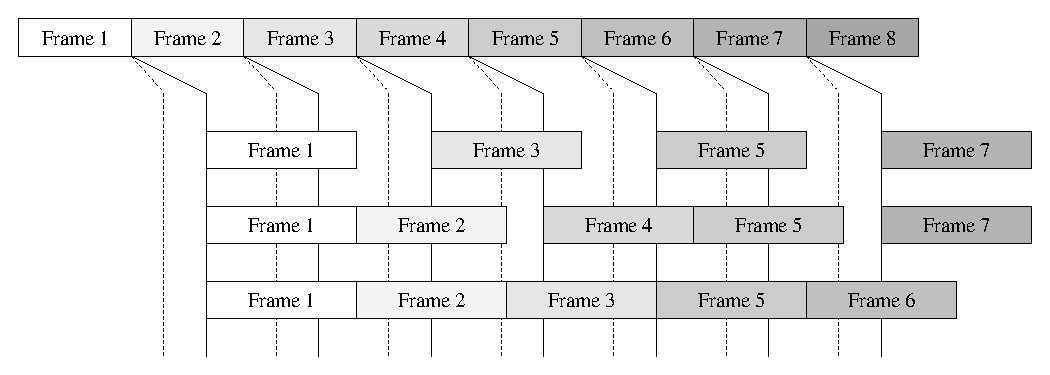
\includegraphics[width=\columnwidth]{fig-throughput-nowait}
\caption{
The top row represents an observable configured for \textit{no-wait};
dashed and solid lines show (exaggerated) start and end times of 
sending an update to three observers, configured as
 \textit{single-buffer},
 \textit{double-buffer},
and \textit{triple-buffer}
respectively.  For the scenario shown, the processing time of the
client is greater than that of the server.
}
\label{fig:throughput-nowait}
\end{figure}


\begin{figure}[t]
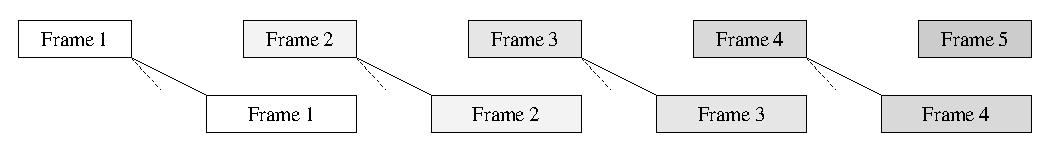
\includegraphics[width=\columnwidth]{fig-throughput-postwait} \\
\ \\
\includegraphics[width=\columnwidth]{fig-throughput-prewait} 
\caption{ 
%
Effect of client behavior on a server.  Four client/server
pairs are shown. In the first, the server is in \textit{wait-after}
mode and the client is in \textit{single-buffer} mode.  In other
words, neither side is willing to drop updates and every update
will get through.
The second pair is similar, except the server is in \textit{wait-before}
mode.  In this case that leads to poor latency, since the communication
delay is long.  For a more realistic ratio of communication delay to
processing time, this choice is in fact preferable.  When the client
is in \textit{double-buffer} or \textit{triple-buffer} mode, then
client processing has no effect on the server, as shown in the lower
pairs.
%
}
\label{fig:throughput-wait}
\end{figure}

\section{Decoupling timing}

Our goal is that observers can be added to an observable without
having an impact on existing observers.  
%
A ``slow'' observer, which takes time to process each update it
received from the observable, should not force a ``fast'' observer of
the same observable to slow down.  This implies either buffering
of messages for bursty channels, or simply dropping messages for
observers that can't keep up.  The second approach is the default
behavior in YARP.

Let us assume we have a ``server'' process which contains an
observable (an output {\tt Port}), and a ``client'' process
which contains a corresponding observer (an input {\tt Port}).
The server process can update the observable in one of three ways:

\begin{itemize} \pflist

\item The default mechanism is \textbf{\textit{no-wait}}.  When the
server process calls the observable's update method ({\it Write}),
then the current state of the observable is made available to be sent
to every free observer, and the server can continue without delay.
Free observers are ones not currently in the process of reading a
previous state of the observable.

\item An alternate mechanism is \textbf{\textit{wait-after}}.  After the same 
steps as {\it no-wait} are taken, the server can choose
to wait for all communication to cease before continuing (by 
calling {\it FinishSend}).  This guarantees that all observers will
be notified and free to receive the next update.

\item The final mechanism is \textbf{\textit{wait-before}}.  The server can choose
to wait for all communication to cease before updating (by calling a
blocking version of {\it Write}).  This guarantees that all observers
will be free, and the update will be sent to all of them.  The
difference between this and {\it wait-after} is that, if the processing
time of the server (the time between updates) is greater than the time 
taken to send the update to all observers, then the server will never
actually need to wait.

\end{itemize}

\noindent
%
To insulate the server from the details of implementing all this, the
state associated with an observable is made logically distinct from
the observable itself, and once an update is requested (by a call to
{\em Write}) the state becomes the property of the communication
system, while the server is given a replacement object to work with.
%
The communication system manages a pool of such state objects which
grows to whatever size is necessary based on the speed of the various
observers.
%

On the client side, there are some choices in how the
observer behaves:

\begin{itemize} \pflist

\item \textbf{\textit{triple-buffer}} behavior: an observer becomes free for
another update immediately after having received one, before any
processing is done by the client.  If updates arrive faster than
processing occurs, then updates will be lost from time to time (where
``lost'' means ``never processed''), but the most recent update
received will always be available to the client immediately when processing
is completed.

\item \textbf{\textit{double-buffer}} behavior: same as above, but if
an update is currently arriving, then no new content will be available
to the client until the update arrives.  This is good if it is better
to minimize latency of non-dropped updates than to maximize
throughput.

\item \textbf{\textit{single-buffer}} behavior: the arrival of updates
is delayed until the client completes processing.  No updates will ever be 
lost on the client side.


\end{itemize}

\noindent The default behavior for YARP is \textit{no-wait} for
the observable (server side) and \textit{triple-buffer} for 
the observer (client side).  This
choice minimizes the time spent waiting for communication to occur by
the server and the client, and permits updates to be lost (either by
never sending them, or discarding them on the client side) if the
client is not keeping up.  This is generally a good choice for
real-time performance.

The default of \textit{no-wait} on the server side is particularly
important, since it minimizes coupling between observers of the same
observable.  If it is important that updates are never lost, then
inevitably there will be coupling, since a slow client can then force
the server to slow down the rate at which it serves all clients.
See Figure~\ref{fig:throughput-nowait}.

The default of \textit{triple-buffer} on the client side insulates the
server from the client's behavior by default.  Even if the server is
configured to wait, default clients will only delay the server
with the time taken to communicate with them, and not the time
they take to process the update.  Clients which absolutely
need a guarantee of zero update loss can choose \textit{single-buffer}
behavior.  See Figure~\ref{fig:throughput-wait}.


